\documentclass[aspectratio=169]{beamer}
\usetheme{metropolis}
\usecolortheme{crane}

\usepackage{amsmath, amssymb}
\usepackage{tikz}
\usepackage{xcolor}
\usepackage{fontawesome5}

\usetikzlibrary{trees, positioning, arrows.meta, shapes.geometric}

% Custom colors for red-black trees
\definecolor{rbred}{RGB}{220, 38, 127}
\definecolor{rbblack}{RGB}{33, 33, 33}
\definecolor{rbgray}{RGB}{200, 200, 200}

% TikZ styles for tree nodes
\tikzset{
    rbnode/.style={circle, draw, thick, minimum size=8mm, font=\small\bfseries},
    rednode/.style={rbnode, fill=rbred!20, text=rbred, draw=rbred},
    blacknode/.style={rbnode, fill=rbblack!10, text=rbblack, draw=rbblack},
    nilnode/.style={rbnode, fill=rbgray!30, text=rbgray, draw=rbgray, minimum size=6mm}
}

\title{Red-Black Trees}
\subtitle{Why Even the Inventor Moved On...}
\author{Your Name}
\date{\today}

\begin{document}

% Part 1: Introduction to Insertion warning
% ══════════════════════════════════════════════════════════════
% SLIDE 1: Store and Search Data
% ══════════════════════════════════════════════════════════════
\begin{frame}{We Need to Store and Search Data}
    \vspace{0.5cm}
    \begin{itemize}
        \item<1-> \large Everything is \textbf{tree-structured}
        \item<2-> \large \textbf{Insert} data into the structure
        \item<3-> \large \textbf{Delete} data efficiently
        \item<4-> \large \textbf{Search} for data quickly
    \end{itemize}
\end{frame}

% ══════════════════════════════════════════════════════════════
% SLIDE 1B: Question
% ══════════════════════════════════════════════════════════════
\begin{frame}
    \vspace{2cm}
    \begin{center}
        \Huge Good way to do all of this?
    \end{center}
\end{frame}

% ══════════════════════════════════════════════════════════════
% SLIDE 1C: Answer
% ══════════════════════════════════════════════════════════════
\begin{frame}
    \vspace{2.5cm}
    \begin{center}
        \only<1>{\Huge\textcolor{goodgreen}{\textbf{Use a BST!}}}
    \end{center}
\end{frame}



% ══════════════════════════════════════════════════════════════
% SLIDE 2: BST Rule
% ══════════════════════════════════════════════════════════════
\begin{frame}{The BST Rule}
    \begin{columns}[c]
        \column{0.5\textwidth}
            \vspace{0.3cm}
            \begin{center}
                \large How does BST decide where to put a node?
            \end{center}
            \vspace{0.5cm}
            \begin{itemize}
                \item<2-> \textbf{Smaller than me?} Go \textcolor{goodgreen}{\textbf{Left}}
                \item<4-> \textbf{Larger than me?} Go \textcolor{rbred}{\textbf{Right}}
            \end{itemize}

        \column{0.48\textwidth}
            \only<1->{
                \begin{center}
                \begin{tikzpicture}[scale=1, every node/.style={transform shape}]
                    % Start with tree with 5-6 nodes
                    \only<1>{
                        \node[bstnode] (root) at (0,0) {20};
                        \node[bstnode] (l15) at (-1.5,-1.2) {15};
                        \node[bstnode] (r30) at (1.5,-1.2) {30};
                        \node[bstnode] (ll12) at (-2.2,-2.4) {12};
                        \node[bstnode] (lr18) at (-0.8,-2.4) {18};
                        \node[bstnode] (rr35) at (2.2,-2.4) {35};
                        
                        \draw[thick] (root) -- (l15);
                        \draw[thick] (root) -- (r30);
                        \draw[thick] (l15) -- (ll12);
                        \draw[thick] (l15) -- (lr18);
                        \draw[thick] (r30) -- (rr35);
                    }
                    
                    % Add 10 to left - show floating then directly attached
                    \only<2>{
                        \node[bstnode] (root) at (0,0) {20};
                        \node[bstnode, fill=goodgreen!40, draw=goodgreen, thick] (new10) at (-1.5,1.5) {10};
                        \node[below=0.05cm of new10, font=\scriptsize, text=goodgreen] {new};
                    }
                    \only<3>{
                        \node[bstnode] (root) at (0,0) {20};
                        \node[bstnode, fill=goodgreen!30, draw=goodgreen] (l10) at (-1.2,-1.2) {10};
                        \draw[thick, goodgreen] (root) -- (l10);
                    }
                    
                    % Add 25 to right - show floating then directly attached
                    \only<4>{
                        \node[bstnode] (root) at (0,0) {20};
                        \node[bstnode] (l10) at (-1.2,-1.2) {10};
                        \draw[thick] (root) -- (l10);
                        \node[bstnode, fill=rbred!40, draw=rbred, thick] (new25) at (1.5,1.5) {25};
                        \node[below=0.05cm of new25, font=\scriptsize, text=rbred] {new};
                    }
                    \only<5>{
                        \node[bstnode] (root) at (0,0) {20};
                        \node[bstnode] (l10) at (-1.2,-1.2) {10};
                        \node[bstnode, fill=rbred!30, draw=rbred] (r25) at (1.2,-1.2) {25};
                        \draw[thick] (root) -- (l10);
                        \draw[thick, rbred] (root) -- (r25);
                    }
                    
                    % Final full tree
                    \only<6->{
                        \node[bstnode] (root) at (0,-0.5) {20};
                        \node[bstnode] (l10) at (-1.5,-1.7) {10};
                        \node[bstnode] (r30) at (1.5,-1.7) {30};
                        \node[bstnode] (ll5) at (-2.2,-2.9) {5};
                        \node[bstnode] (lr15) at (-0.8,-2.9) {15};
                        \node[bstnode] (rl25) at (0.8,-2.9) {25};
                        \node[bstnode] (rr35) at (2.2,-2.9) {35};
                        
                        \draw[thick] (root) -- (l10);
                        \draw[thick] (root) -- (r30);
                        \draw[thick] (l10) -- (ll5);
                        \draw[thick] (l10) -- (lr15);
                        \draw[thick] (r30) -- (rl25);
                        \draw[thick] (r30) -- (rr35);
                    }
                \end{tikzpicture}
                \end{center}
            }
    \end{columns}
    
    \only<6->{
        \vspace{0.3cm}
        \begin{center}
            \Large\textbf{Good technique!}
        \end{center}
    }
\end{frame}

% ══════════════════════════════════════════════════════════════
% SLIDE 3 (Page 6): Insert Roll Numbers - Title
% ══════════════════════════════════════════════════════════════
\begin{frame}{Insert the roll numbers in a class sequentially}
    \begin{center}
        \large 1, 2, 3, 4 \ldots 10
    \end{center}
    \vspace{0.3cm}
\end{frame}

% ══════════════════════════════════════════════════════════════
% SLIDE 4 (Page 7): Goes to Right
% ══════════════════════════════════════════════════════════════
\begin{frame}{Insert the roll numbers in a class sequentially}
    \begin{center}
        \large 1, 2, 3, 4 \ldots 10
    \end{center}
    \vspace{0.3cm}
    \begin{columns}[c]
        \column{0.45\textwidth}
            \begin{itemize}
                \item Each goes to the \textcolor{rbred}{\textbf{right}} of the last
            \end{itemize}

        \column{0.52\textwidth}
            \begin{center}
            \begin{tikzpicture}[scale=0.7,
                every node/.style={},
            ]
                \node[bstnode] (n1) at (0,0) {1};
                \node[bstnode] (n2) at (1,-1.3) {2}; \draw[thick,->] (n1) -- (n2);
                \node[bstnode] (n3) at (2,-2.6) {3}; \draw[thick,->] (n2) -- (n3);
            \end{tikzpicture}
            \end{center}
    \end{columns}
\end{frame}

% ══════════════════════════════════════════════════════════════
% SLIDE 5 (Page 8): Keeps Growing
% ══════════════════════════════════════════════════════════════
\begin{frame}{Insert the roll numbers in a class sequentially}
    \begin{center}
        \large 1, 2, 3, 4 \ldots 10
    \end{center}
    \vspace{0.3cm}
    \begin{columns}[c]
        \column{0.45\textwidth}
            \begin{itemize}
                \item Each goes to the \textcolor{rbred}{\textbf{right}} of the last
                \item The tree just keeps \textcolor{accent}{\textbf{growing}} right\ldots
            \end{itemize}

        \column{0.52\textwidth}
            \begin{center}
            \begin{tikzpicture}[scale=0.75,
                every node/.style={},
            ]
                \node[bstnode] (n1) at (0,0) {1};
                \node[bstnode] (n2) at (1,-1.3) {2}; \draw[thick,->] (n1) -- (n2);
                \node[bstnode] (n3) at (2,-2.6) {3}; \draw[thick,->] (n2) -- (n3);
                \node[bstnode] (n4) at (3,-3.9) {4}; \draw[thick,->] (n3) -- (n4);
                \node[bstnode] (n5) at (4,-5.2) {5}; \draw[thick,->] (n4) -- (n5);
                \node[below right=0.5cm and 0.3cm of n5, font=\normalsize, text=rbred] {\textbf{\ldots and on}};
            \end{tikzpicture}
            \end{center}
    \end{columns}
\end{frame}

% ══════════════════════════════════════════════════════════════
% SLIDE 6 (Page 9): Still Works
% ══════════════════════════════════════════════════════════════
\begin{frame}{Insert the roll numbers in a class sequentially}
    \begin{center}
        \large 1, 2, 3, 4 \ldots 10
    \end{center}
    \vspace{0.3cm}
    \begin{columns}[c]
        \column{0.45\textwidth}
            \begin{itemize}
                \item Each goes to the \textcolor{rbred}{\textbf{right}} of the last
                \item The tree just keeps \textcolor{accent}{\textbf{growing}} right\ldots
            \end{itemize}

        \column{0.52\textwidth}
            \begin{center}
            \begin{tikzpicture}[scale=0.75,
                every node/.style={},
            ]
                \node[bstnode] (n1) at (0,0) {1};
                \node[bstnode] (n2) at (1,-1.3) {2}; \draw[thick,->] (n1) -- (n2);
                \node[bstnode] (n3) at (2,-2.6) {3}; \draw[thick,->] (n2) -- (n3);
                \node[bstnode] (n4) at (3,-3.9) {4}; \draw[thick,->] (n3) -- (n4);
                \node[bstnode] (n5) at (4,-5.2) {5}; \draw[thick,->] (n4) -- (n5);
                \node[below right=0.5cm and 0.3cm of n5, font=\normalsize, text=rbred] {\textbf{\ldots and on}};
            \end{tikzpicture}
            \end{center}
    \end{columns}
    
    \vspace{-0.7cm}
    \begin{center}
        \Large\textbf{Still works!}
    \end{center}
\end{frame}

% ══════════════════════════════════════════════════════════════
% SLIDE 7 (Pages 10-14): Problem Points
% ══════════════════════════════════════════════════════════════
\begin{frame}{But, What's the Problem?}
    \vspace{0.3cm}
    \begin{columns}[c]
        \column{0.45\textwidth}
            \begin{itemize}
                \item<1-> \textcolor{badred}{\textbf{Height becomes $n$}}
                \item<2-> Insertion takes $O(n)$
                \item<3-> Deletion takes $O(n)$
                \item<4-> Search takes $O(n)$
                \item<5-> A linked list in disguise
            \end{itemize}

        \column{0.52\textwidth}
            \begin{center}
            \begin{tikzpicture}[scale=0.75,
                every node/.style={},
            ]
                \node[bstnode] (n1) at (0,0) {1};
                \node[bstnode] (n2) at (1,-1.3) {2}; \draw[thick,->] (n1) -- (n2);
                \node[bstnode] (n3) at (2,-2.6) {3}; \draw[thick,->] (n2) -- (n3);
                \node[bstnode] (n4) at (3,-3.9) {4}; \draw[thick,->] (n3) -- (n4);
                \node[bstnode] (n5) at (4,-5.2) {5}; \draw[thick,->] (n4) -- (n5);
                \node[below right=0.5cm and 0.3cm of n5, font=\normalsize, text=rbred] {\textbf{\ldots and on}};
            \end{tikzpicture}
            \end{center}
    \end{columns}
\end{frame}

% ══════════════════════════════════════════════════════════════
% SLIDE 12 (Page 15): Time Complexity
% ══════════════════════════════════════════════════════════════
\begin{frame}{But, What's the Problem?}
    \vspace{0.6cm}
    \begin{itemize}
        \item Insertion takes $O(n)$
        \item Deletion takes $O(n)$
        \item Search takes $O(n)$
        \item A linked list in disguise
    \end{itemize}
    \vspace{0.6cm}
    \begin{center}
        \Large\textbf{Time complexity becomes $O(n)$}
    \end{center}
\end{frame}

% ══════════════════════════════════════════════════════════════
% SLIDE 5 (Page 12): Solution - Definition
% ══════════════════════════════════════════════════════════════
\begin{frame}{The Solution?}
    \vspace{1cm}
    \begin{center}
        \Large Use a BST that \textbf{promises} to keep its height \textcolor{goodgreen}{\textbf{logarithmic}}\\[0.3cm]
        \large no matter how and what element you insert.
    \end{center}
\end{frame}

% ══════════════════════════════════════════════════════════════
% SLIDE 6 (Page 13): Self-Balancing Trees Examples
% ══════════════════════════════════════════════════════════════
\begin{frame}{The Solution?}
    \vspace{0.5cm}
    \large Examples of Self-Balancing Trees:
    \vspace{0.5cm}
    \begin{itemize}
        \item<1-> AVL Tree
        \item<2-> \textbf{\textcolor{rbred}{Red-Black Tree}}
        \item<3-> Splay Tree
        \item<4-> B-Tree
    \end{itemize}
\end{frame}

% ══════════════════════════════════════════════════════════════
% SLIDE 7 (Page 14): Let's Look at RBT
% ══════════════════════════════════════════════════════════════
\begin{frame}
    \vspace{0.5cm}
    \begin{center}
        \LARGE Let's look at \textcolor{rbred}{Red}-\textbf{Black} Trees
        
        \vspace{0.5cm}
        \includegraphics[height=5cm]{images/magnifying_glass.png}
    \end{center}
\end{frame}

% ══════════════════════════════════════════════════════════════
% SLIDE 8 (Page 15): What is Red-Black Tree
% ══════════════════════════════════════════════════════════════
\begin{frame}{What is Red-Black Tree}
    \vspace{1.5cm}
    \begin{center}
        \Large A Red-Black Tree rebalances itself by coloring nodes \textcolor{rbred}{\textbf{red}} and \textbf{black}, ensuring no two \textcolor{rbred}{\textbf{red}} nodes are {\textbf{adjacent}} and all {\textbf{paths}} have the same \textbf{black-height}, which keeps its height \textcolor{goodgreen}{\textbf{logarithmic}}.
    \end{center}
    \only<2->{
        \vspace{1cm}
        \begin{center}
            \Large\textcolor{blue!80!black}{\textbf{Height becomes log(n) here!}}
        \end{center}
    }
\end{frame}

% ══════════════════════════════════════════════════════════════
% SLIDE (Page 16): Five Points to Remember - Title
% ══════════════════════════════════════════════════════════════
\begin{frame}{How does RBT do it:Properties}
    \vspace{1.5cm}
    \begin{center}
        \Large\textbf{Five points to remember}
    \end{center}
\end{frame}

% ══════════════════════════════════════════════════════════════
% SLIDE (Page 17): Property 1 — Red or Black with Hence line
% ══════════════════════════════════════════════════════════════
\begin{frame}{How does RBT do it:Properties}
    \vspace{1cm}
    \begin{itemize}
        \item \textbf{Property 1:} Every node is either \textcolor{rbred}{red} or black
    \end{itemize}
    \only<2->{
        \vspace{1cm}
        \begin{center}
            \textbf{Hence, the name \textcolor{rbred}{Red} Black Tree}
        \end{center}
    }
\end{frame}

% ══════════════════════════════════════════════════════════════
% SLIDE 9 (Page 18): Property 2 — Root is Black (with right/wrong)
% ══════════════════════════════════════════════════════════════
\begin{frame}{How does RBT do it:Properties}
    \begin{itemize}
        \item \textbf{Property 2:} Root will always be a black node
    \end{itemize}
    \vspace{0.5cm}
    \begin{columns}[c]
        \column{0.5\textwidth}
            \begin{center}
            \only<2->{
                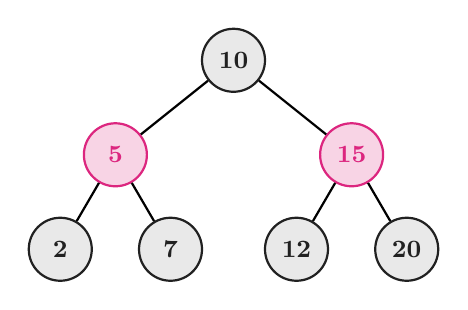
\begin{tikzpicture}[scale=1]
                    \node[blacknode] (root) at (0,-0.5) {10};
                    \node[rednode] (l5) at (-1.5,-1.7) {5};
                    \node[rednode] (r15) at (1.5,-1.7) {15};
                    \node[blacknode] (ll2) at (-2.2,-2.9) {2};
                    \node[blacknode] (lr7) at (-0.8,-2.9) {7};
                    \node[blacknode] (rl12) at (0.8,-2.9) {12};
                    \node[blacknode] (rr20) at (2.2,-2.9) {20};
                    
                    \draw[thick] (root) -- (l5);
                    \draw[thick] (root) -- (r15);
                    \draw[thick] (l5) -- (ll2);
                    \draw[thick] (l5) -- (lr7);
                    \draw[thick] (r15) -- (rl12);
                    \draw[thick] (r15) -- (rr20);
                \end{tikzpicture}
            }
            
            \only<4->{\vspace{0.3cm}\textcolor{goodgreen}{\textbf{Correct}}}
            \end{center}
        
        \column{0.5\textwidth}
            \begin{center}
            \only<3->{
                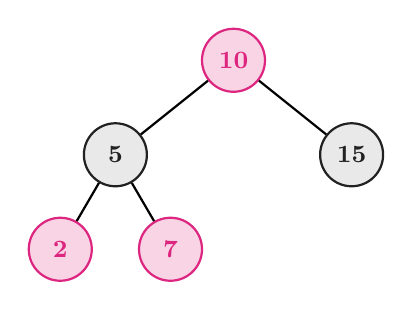
\begin{tikzpicture}[scale=1]
                    \node[rednode] (root) at (0,-0.5) {10};
                    \node[blacknode] (l5) at (-1.5,-1.7) {5};
                    \node[blacknode] (r15) at (1.5,-1.7) {15};
                    \node[rednode] (ll2) at (-2.2,-2.9) {2};
                    \node[rednode] (lr7) at (-0.8,-2.9) {7};
                    
                    \draw[thick] (root) -- (l5);
                    \draw[thick] (root) -- (r15);
                    \draw[thick] (l5) -- (ll2);
                    \draw[thick] (l5) -- (lr7);
                \end{tikzpicture}
            }
            
            \only<5->{\vspace{0.3cm}\textcolor{badred}{\textbf{Incorrect}}}
            \end{center}
    \end{columns}
\end{frame}

% ══════════════════════════════════════════════════════════════
% SLIDE 10 (Page 19): Property 3 — Leaves are Black / NIL
% ══════════════════════════════════════════════════════════════
\begin{frame}{How does RBT do it:Properties}
    \begin{itemize}
        \item \textbf{Property 3:} Leaves will either be black or NIL
    \end{itemize}
    \vspace{0.3cm}
    \begin{columns}[c]
        \column{0.5\textwidth}
            \begin{center}
            \only<2->{
                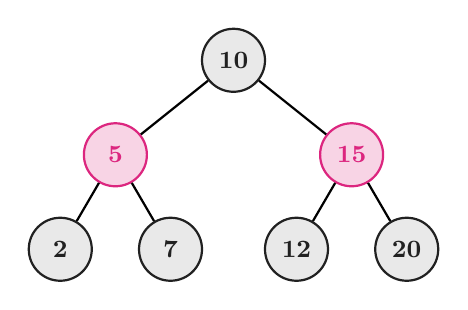
\begin{tikzpicture}[scale=1]
                    \node[blacknode] (root) at (0,-0.5) {10};
                    \node[rednode] (l5) at (-1.5,-1.7) {5};
                    \node[rednode] (r15) at (1.5,-1.7) {15};
                    \node[blacknode] (ll2) at (-2.2,-2.9) {2};
                    \node[blacknode] (lr7) at (-0.8,-2.9) {7};
                    \node[blacknode] (rl12) at (0.8,-2.9) {12};
                    \node[blacknode] (rr20) at (2.2,-2.9) {20};
                    
                    \draw[thick] (root) -- (l5);
                    \draw[thick] (root) -- (r15);
                    \draw[thick] (l5) -- (ll2);
                    \draw[thick] (l5) -- (lr7);
                    \draw[thick] (r15) -- (rl12);
                    \draw[thick] (r15) -- (rr20);
                \end{tikzpicture}
                
                \only<4->{\vspace{0.2cm}\small\textbf{Black Leaves}}
            }
            \end{center}
        
        \column{0.5\textwidth}
            \begin{center}
            \only<3->{
                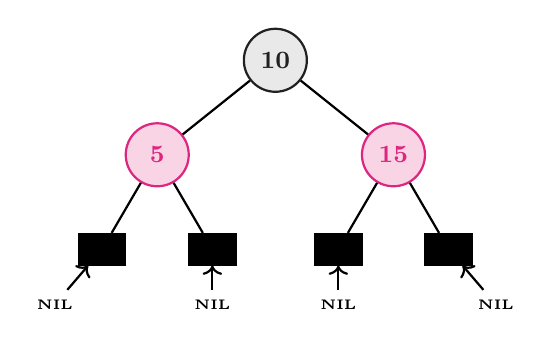
\begin{tikzpicture}[scale=1]
                    \node[blacknode] (root) at (0,-0.5) {10};
                    \node[rednode] (l5) at (-1.5,-1.7) {5};
                    \node[rednode] (r15) at (1.5,-1.7) {15};
                    % NIL nodes as rectangles
                    \node[rectangle, fill=black, draw=black, minimum width=6mm, minimum height=4mm] (n1) at (-2.2,-2.9) {};
                    \node[rectangle, fill=black, draw=black, minimum width=6mm, minimum height=4mm] (n2) at (-0.8,-2.9) {};
                    \node[rectangle, fill=black, draw=black, minimum width=6mm, minimum height=4mm] (n3) at (0.8,-2.9) {};
                    \node[rectangle, fill=black, draw=black, minimum width=6mm, minimum height=4mm] (n4) at (2.2,-2.9) {};
                    
                    \draw[thick] (root) -- (l5);
                    \draw[thick] (root) -- (r15);
                    \draw[thick] (l5) -- (n1);
                    \draw[thick] (l5) -- (n2);
                    \draw[thick] (r15) -- (n3);
                    \draw[thick] (r15) -- (n4);
                    
                    % NIL labels with arrows
                    \node[font=\tiny\bfseries] (lbl1) at (-2.8,-3.6) {NIL};
                    \node[font=\tiny\bfseries] (lbl2) at (-0.8,-3.6) {NIL};
                    \node[font=\tiny\bfseries] (lbl3) at (0.8,-3.6) {NIL};
                    \node[font=\tiny\bfseries] (lbl4) at (2.8,-3.6) {NIL};
                    \draw[->, thick, black] (lbl1) -- (n1);
                    \draw[->, thick, black] (lbl2) -- (n2);
                    \draw[->, thick, black] (lbl3) -- (n3);
                    \draw[->, thick, black] (lbl4) -- (n4);
                \end{tikzpicture}
                
                \only<5->{\vspace{0.2cm}\small\textbf{NIL nodes (counted as Black)}}
            }
            \end{center}
    \end{columns}
\end{frame}

% ══════════════════════════════════════════════════════════════
% SLIDE 11 (Page 20): Property 4 — No Two Consecutive Red
% ══════════════════════════════════════════════════════════════
\begin{frame}{How does RBT do it:Properties}
    \begin{itemize}
        \item \textbf{Property 4:} There will be no two consecutive red nodes
    \end{itemize}
    \vspace{0.3cm}
    \begin{columns}[c]
        \column{0.5\textwidth}
            \begin{center}
            \only<2->{
                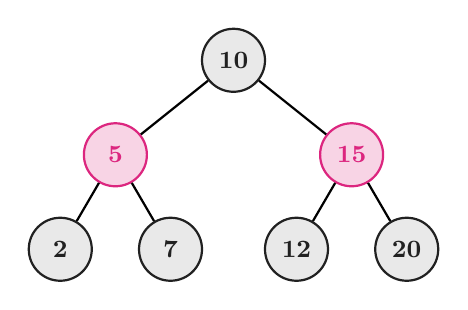
\begin{tikzpicture}[scale=1]
                    \node[blacknode] (root) at (0,-0.5) {10};
                    \node[rednode] (l5) at (-1.5,-1.7) {5};
                    \node[rednode] (r15) at (1.5,-1.7) {15};
                    \node[blacknode] (ll2) at (-2.2,-2.9) {2};
                    \node[blacknode] (lr7) at (-0.8,-2.9) {7};
                    \node[blacknode] (rl12) at (0.8,-2.9) {12};
                    \node[blacknode] (rr20) at (2.2,-2.9) {20};
                    
                    \draw[thick] (root) -- (l5);
                    \draw[thick] (root) -- (r15);
                    \draw[thick] (l5) -- (ll2);
                    \draw[thick] (l5) -- (lr7);
                    \draw[thick] (r15) -- (rl12);
                    \draw[thick] (r15) -- (rr20);
                \end{tikzpicture}
            }
            
            \only<4->{\vspace{0.3cm}\textcolor{goodgreen}{\textbf{Correct}}}
            \end{center}
        
        \column{0.5\textwidth}
            \begin{center}
            \only<3->{
                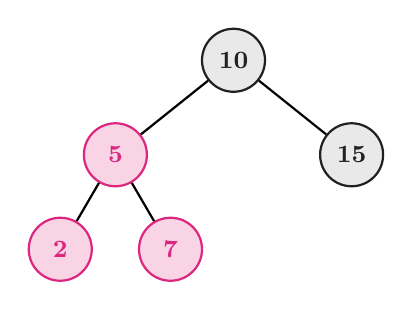
\begin{tikzpicture}[scale=1]
                    \node[blacknode] (root) at (0,-0.5) {10};
                    \node[rednode] (l5) at (-1.5,-1.7) {5};
                    \node[blacknode] (r15) at (1.5,-1.7) {15};
                    \node[rednode] (ll2) at (-2.2,-2.9) {2};
                    \node[rednode] (lr7) at (-0.8,-2.9) {7};
                    
                    \draw[thick] (root) -- (l5);
                    \draw[thick] (root) -- (r15);
                    \draw[thick] (l5) -- (ll2);
                    \draw[thick] (l5) -- (lr7);
                \end{tikzpicture}
            }
            
            \only<5->{\vspace{0.3cm}\textcolor{badred}{\textbf{Incorrect}}}
            \end{center}
    \end{columns}
\end{frame}

% ══════════════════════════════════════════════════════════════
% SLIDE 12 (Page 21): Property 5 — Equal Black Height
% ══════════════════════════════════════════════════════════════
\begin{frame}{How does RBT do it:Properties}
    \begin{itemize}
        \item \textbf{Property 5:} From a given node, the number of black nodes in any given path will always be same for that node
    \end{itemize}
    \vspace{0.2cm}
    \only<2->{
        \begin{center}
        \begin{tikzpicture}[scale=0.9]
            % Big RBT tree - wider spacing
            \node[blacknode] (root) at (0,0) {20};
            \node[rednode] (l10) at (-3,-1.3) {10};
            \node[rednode] (r30) at (3,-1.3) {30};
            \node[blacknode] (ll5) at (-4.5,-2.6) {5};
            \node[blacknode] (lr15) at (-1.5,-2.6) {15};
            \node[blacknode] (rl25) at (1.5,-2.6) {25};
            \node[blacknode] (rr35) at (4.5,-2.6) {35};
            
            \draw[thick] (root) -- (l10);
            \draw[thick] (root) -- (r30);
            \draw[thick] (l10) -- (ll5);
            \draw[thick] (l10) -- (lr15);
            \draw[thick] (r30) -- (rl25);
            \draw[thick] (r30) -- (rr35);
            
            % Path 1: root -> 10 -> 5
            \only<3->{
                \draw[line width=2.5pt, orange!80!black] (root) -- (l10) -- (ll5);
                \node[below=0.15cm of ll5, font=\scriptsize, text=orange!80!black] {\textbf{bc=2}};
            }
            
            % Path 2: root -> 10 -> 15
            \only<4->{
                \draw[line width=2.5pt, green!60!black] (root) -- (l10) -- (lr15);
                \node[below=0.15cm of lr15, font=\scriptsize, text=green!60!black] {\textbf{bc=2}};
            }
            
            % Path 3: root -> 30 -> 25
            \only<5->{
                \draw[line width=2.5pt, red!70!black] (root) -- (r30) -- (rl25);
                \node[below=0.15cm of rl25, font=\scriptsize, text=red!70!black] {\textbf{bc=2}};
            }
            
            % Path 4: root -> 30 -> 35
            \only<6->{
                \draw[line width=2.5pt, blue!70!black] (root) -- (r30) -- (rr35);
                \node[below=0.15cm of rr35, font=\scriptsize, text=blue!70!black] {\textbf{bc=2}};
            }
        \end{tikzpicture}
        \end{center}
    }
    \only<7->{
        \begin{center}
            \textbf{All paths from root have same black count = 2}
        \end{center}
    }
\end{frame}

% ══════════════════════════════════════════════════════════════
% SLIDE (Page 22): RBT Operations Intro
% ══════════════════════════════════════════════════════════════
\begin{frame}{RBT Operations}
    \vspace{1cm}
    Now, How do these points ensure the "rebalancing" feature of Red Black Tree?
    
    \only<2->{
        \vspace{2cm}
        \begin{center}
            \Large\textbf{Let's see some operations....}
        \end{center}
    }
\end{frame}

% ══════════════════════════════════════════════════════════════
% SLIDE: Insertion Title
% ══════════════════════════════════════════════════════════════
\begin{frame}{Insertion}
\end{frame}


% Part 2a: Insertion
% ============================================================
% part2a_insertion.tex  –  Red-Black Tree: Insertion
% ============================================================

% ── Insertion process ──────────────────────────────────────
\begin{frame}{Insertion: The Process}
    \begin{enumerate}
        \item<1-> Insert like a normal BST
        \item<2-> Color the new node \textcolor{rbred}{\textbf{RED}}
        \item<3-> Fix any violations
    \end{enumerate}

    \only<4->{
        \begin{center}
            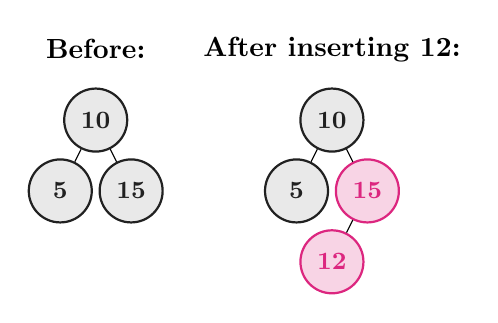
\begin{tikzpicture}[scale=0.6]
                \node at (-2.5,1.5) {\textbf{Before:}};
                \node[blacknode] at (-2.5,0) {10}
                    child {node[blacknode] {5}}
                    child {node[blacknode] {15}};

                \node at (2.5,1.5) {\textbf{After inserting 12:}};
                \node[blacknode] at (2.5,0) {10}
                    child {node[blacknode] {5}}
                    child {node[rednode]  {15}
                        child {node[rednode]{12}}
                        child[missing] {}
                    };
            \end{tikzpicture}
        \end{center}
    }

    \only<5->{
        \begin{alertblock}{Problem!}
            Two adjacent red nodes — Property 4 violated!
        \end{alertblock}
    }
\end{frame}

% ── Fixing violations ──────────────────────────────────────
\begin{frame}{Fixing Violations}
    \begin{columns}
        \column{0.5\textwidth}
        \begin{block}{Uncle is RED}
            \begin{itemize}
                \item Easy case!
                \item Just recolor
                \item Flip parent, uncle \& grandparent
            \end{itemize}
        \end{block}

        \pause

        \column{0.5\textwidth}
        \begin{alertblock}{Uncle is BLACK}
            \begin{itemize}
                \item Hard case!
                \item Need rotations
                \item Left rotate, right rotate
                \item Sometimes both!
            \end{itemize}
        \end{alertblock}
    \end{columns}

    \pause
    \vspace{0.4cm}

    \begin{center}
        \Large\textcolor{rbred}{This is where it gets tricky!}\\[0.3cm]
        \large But it keeps the tree balanced!
    \end{center}
\end{frame}

% ── Remember the linked-list problem? ──────────────────────
\begin{frame}{Remember This Problem?}
    \begin{center}
        \Large Let's try inserting \textbf{1, 2, 3, 4, 5} again\ldots\\[0.3cm]
        \large But this time in a \textcolor{rbred}{Red-Black Tree}!
    \end{center}

    \pause

    \begin{columns}
        \column{0.5\textwidth}
        \begin{block}{Regular BST}
            Became a linked list\\
            Height $= 5$\\
            $O(n)$ operations \textcolor{rbred}{\faIcon{sad-tear}}
        \end{block}

        \column{0.5\textwidth}
        \pause
        \begin{alertblock}{Red-Black Tree}
            Let's see what happens\ldots\\
            Will it stay balanced?\\
            \textcolor{green!70!black}{\faIcon{magic}} Stay tuned!
        \end{alertblock}
    \end{columns}

    \vspace{0.4cm}
    \pause

    \begin{center}
        \Large\textbf{Watch the magic happen!}
    \end{center}
\end{frame}

% ── Simulation progress bar helper ─────────────────────────
% Drawn at the bottom of each simulation frame
\newcommand{\simProgress}[2]{%
    % #1 = current step (1-5), #2 = label text
    \begin{tikzpicture}[scale=1]
        \foreach \i in {1,...,5}{
            \pgfmathsetmacro{\done}{(\i<=#1)?1:0}
            \ifnum\i=#1
                \node[circle, draw=rbred, fill=rbred, text=white,
                      inner sep=2pt, minimum size=18pt,
                      font=\bfseries\small] at (\i*0.9,0) {\i};
            \else
                \ifnum\i<#1
                    \node[circle, draw=green!60!black, fill=green!60!black,
                          text=white, inner sep=2pt, minimum size=18pt,
                          font=\small] at (\i*0.9,0) {\checkmark};
                \else
                    \node[circle, draw=gray!50, fill=gray!15, text=gray,
                          inner sep=2pt, minimum size=18pt,
                          font=\small] at (\i*0.9,0) {\i};
                \fi
            \fi
        }
        \draw[gray!40,thick] (0.9,0) -- (4.5,0);
    \end{tikzpicture}%
    \quad\textcolor{gray}{\small #2}%
}

% ── Step 1: Insert 1 ───────────────────────────────────────
\begin{frame}{Simulation — Step 1 of 5: Insert \textbf{1}}

    \begin{center}
        \simProgress{1}{Inserting 1}
    \end{center}

    \vspace{0.3cm}

    \begin{columns}
        \column{0.55\textwidth}
        \begin{itemize}
            \item<1-> First node is always the root
            \item<2-> Color it \textcolor{rbblack}{\textbf{BLACK}}
            \item<3-> Property 2: Root must be black \textcolor{green!70!black}{\faIcon{check}}
        \end{itemize}

        \column{0.45\textwidth}
        \only<2->{
            \begin{center}
                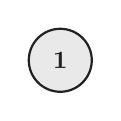
\begin{tikzpicture}
                    \node[blacknode] {1};
                \end{tikzpicture}
            \end{center}
        }
    \end{columns}

    \vspace{0.3cm}
    \only<3->{
        \begin{block}{\faIcon{check-circle}\; All properties satisfied!}
            Height $= 1$\quad Black-height $= 1$
        \end{block}
    }
\end{frame}

% ── Step 2: Insert 2 ───────────────────────────────────────
\begin{frame}{Simulation — Step 2 of 5: Insert \textbf{2}}

    \begin{center}
        \simProgress{2}{Inserting 2}
    \end{center}

    \vspace{0.3cm}

    \begin{columns}
        \column{0.55\textwidth}
        \begin{itemize}
            \item<1-> Insert as right child of 1
            \item<2-> Color it \textcolor{rbred}{\textbf{RED}}
            \item<3-> Parent is \textbf{BLACK} $\Rightarrow$ no violation!
        \end{itemize}

        \column{0.45\textwidth}
        \only<2->{
            \begin{center}
                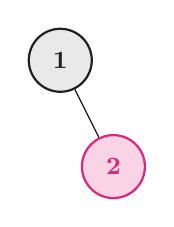
\begin{tikzpicture}[scale=0.9]
                    \node[blacknode] {1}
                        child[missing] {}
                        child {node[rednode] {2}};
                \end{tikzpicture}
            \end{center}
        }
    \end{columns}

    \vspace{0.3cm}
    \only<3->{
        \begin{block}{\faIcon{check-circle}\; Still balanced!}
            Height $= 2$\quad Black-height $= 1$
        \end{block}
    }
\end{frame}

% ── Step 3: Insert 3 ───────────────────────────────────────
\begin{frame}{Simulation — Step 3 of 5: Insert \textbf{3} \textcolor{rbred}{(Fix needed!)}}

    \begin{center}
        \simProgress{3}{Inserting 3 — rotation required}
    \end{center}

    \vspace{0.2cm}

    \begin{columns}[T]
        \column{0.33\textwidth}
        \only<1->{
            \begin{center}
                \textbf{\small After Insert}\\[0.25cm]
                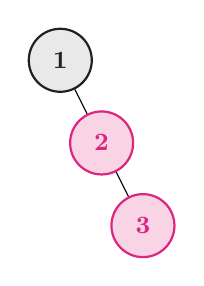
\begin{tikzpicture}[scale=0.7]
                    \node[blacknode] {1}
                        child[missing] {}
                        child {node[rednode] {2}
                            child[missing] {}
                            child {node[rednode] {3}}
                        };
                \end{tikzpicture}\\[0.15cm]
                \fcolorbox{red!80!black}{red!15}{\textcolor{red!70!black}{\bfseries\footnotesize\faIcon{exclamation-triangle}~VIOLATION}}
            \end{center}
        }

        \column{0.33\textwidth}
        \only<2->{
            \begin{center}
                \textbf{\small Left-Rotate at 1}\\[0.25cm]
                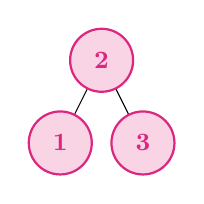
\begin{tikzpicture}[scale=0.7]
                    \node[rednode] {2}
                        child {node[rednode] {1}}
                        child {node[rednode] {3}};
                \end{tikzpicture}\\[0.15cm]
                {\small Rotation complete}
            \end{center}
        }

        \column{0.33\textwidth}
        \only<3->{
            \begin{center}
                \textbf{\small Recolor Root}\\[0.25cm]
                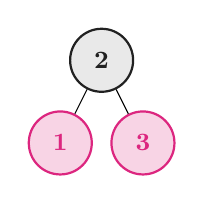
\begin{tikzpicture}[scale=0.7]
                    \node[blacknode] {2}
                        child {node[rednode] {1}}
                        child {node[rednode] {3}};
                \end{tikzpicture}\\[0.15cm]
                \fcolorbox{green!60!black}{green!15}{\textcolor{green!50!black}{\bfseries\footnotesize\faIcon{check-circle}~FIXED}}
            \end{center}
        }
    \end{columns}

    % Animated arrows between diagrams
    \only<2->{\begin{tikzpicture}[remember picture,overlay]
        \draw[->,ultra thick,orange!80!black,bend left=15]
            ([xshift=3.5cm,yshift=3.8cm]current page.south west)
            to node[above,font=\tiny\bfseries]{Rotate}
            ([xshift=6cm,yshift=3.8cm]current page.south west);
    \end{tikzpicture}}
    \only<3->{\begin{tikzpicture}[remember picture,overlay]
        \draw[->,ultra thick,blue!70,bend left=15]
            ([xshift=6.8cm,yshift=3.8cm]current page.south west)
            to node[above,font=\tiny\bfseries]{Recolor}
            ([xshift=9.3cm,yshift=3.8cm]current page.south west);
    \end{tikzpicture}}

    \vspace{0.2cm}
    \only<3->{
        \begin{block}{\faIcon{check-circle}\; Balanced!}
            Height $= 2$\quad (BST would be $3$)
        \end{block}
    }
\end{frame}

% ── Step 4: Insert 4 ───────────────────────────────────────
\begin{frame}{Simulation — Step 4 of 5: Insert \textbf{4}}

    \begin{center}
        \simProgress{4}{Inserting 4 — uncle recolor}
    \end{center}

    \vspace{0.2cm}

    \begin{columns}
        \column{0.5\textwidth}
        \begin{itemize}
            \item<1-> Insert as right child of 3
            \item<2-> Color it \textcolor{rbred}{\textbf{RED}}
            \item<3-> Parent (3) is red — violation!
            \item<4-> Uncle (1) is also red
            \item<5-> Recolor: flip parent, uncle \& grandparent
        \end{itemize}

        \column{0.5\textwidth}
        \only<2-4>{
            \begin{center}
                \textbf{After Insert}\\[0.2cm]
                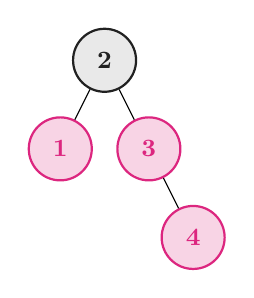
\begin{tikzpicture}[scale=0.75]
                    \node[blacknode] {2}
                        child {node[rednode] {1}}
                        child {node[rednode] {3}
                            child[missing] {}
                            child {node[rednode] {4}}
                        };
                \end{tikzpicture}\\[0.15cm]
                \only<3->{\fcolorbox{red!80!black}{red!15}{\textcolor{red!70!black}{\bfseries\footnotesize\faIcon{exclamation-triangle}~VIOLATION}}}
            \end{center}
        }
        \only<5->{
            \begin{center}
                \textbf{After Recolor}\\[0.2cm]
                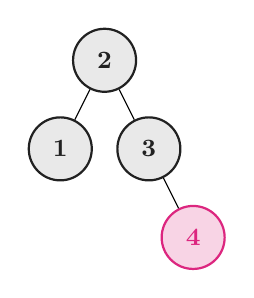
\begin{tikzpicture}[scale=0.75]
                    \node[blacknode] {2}
                        child {node[blacknode] {1}}
                        child {node[blacknode] {3}
                            child[missing] {}
                            child {node[rednode] {4}}
                        };
                \end{tikzpicture}\\[0.15cm]
                \fcolorbox{green!60!black}{green!15}{\textcolor{green!50!black}{\bfseries\footnotesize\faIcon{check-circle}~FIXED}}
            \end{center}
        }
    \end{columns}

    \vspace{0.2cm}
    \only<5->{
        \begin{block}{\faIcon{check-circle}\; Still balanced!}
            Height $= 3$\quad Black-height preserved
        \end{block}
    }
\end{frame}

% ── Step 5: Insert 5 ───────────────────────────────────────
\begin{frame}{Simulation — Step 5 of 5: Insert \textbf{5} \textcolor{rbred}{(Final Fix!)}}

    \begin{center}
        \simProgress{5}{Inserting 5 — rotation + recolor}
    \end{center}

    \vspace{0.2cm}

    \begin{columns}
        \column{0.5\textwidth}
        \begin{itemize}
            \item<1-> Insert as right child of 4
            \item<2-> Color it \textcolor{rbred}{\textbf{RED}}
            \item<3-> Parent (4) is red — violation!
            \item<4-> Uncle is \textbf{BLACK} (NIL)
            \item<5-> Left-rotate at 3, then recolor
        \end{itemize}

        \column{0.5\textwidth}
        \only<2-4>{
            \begin{center}
                \textbf{Before Fix}\\[0.2cm]
                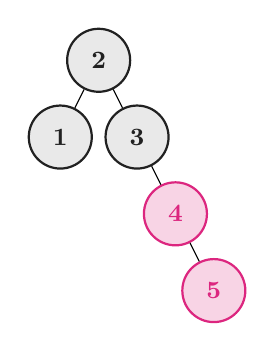
\begin{tikzpicture}[scale=0.65]
                    \node[blacknode] {2}
                        child {node[blacknode] {1}}
                        child {node[blacknode] {3}
                            child[missing] {}
                            child {node[rednode] {4}
                                child[missing] {}
                                child {node[rednode] {5}}
                            }
                        };
                \end{tikzpicture}\\[0.1cm]
                \only<3->{\fcolorbox{red!80!black}{red!15}{\textcolor{red!70!black}{\bfseries\footnotesize\faIcon{exclamation-triangle}~VIOLATION}}}
            \end{center}
        }
        \only<5->{
            \begin{center}
                \textbf{Final Tree}\\[0.2cm]
                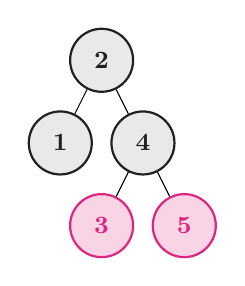
\begin{tikzpicture}[scale=0.7]
                    \node[blacknode] {2}
                        child {node[blacknode] {1}}
                        child {node[blacknode] {4}
                            child {node[rednode] {3}}
                            child {node[rednode] {5}}
                        };
                \end{tikzpicture}\\[0.1cm]
                \fcolorbox{cyan!60!blue}{cyan!10}{\textcolor{cyan!50!blue}{\bfseries\footnotesize\faIcon{star}~PERFECT}}
            \end{center}
        }
    \end{columns}
\end{frame}

% ── Comparison ─────────────────────────────────────────────
\begin{frame}{The Difference is HUGE!}
    \begin{center}
        \Large\textbf{BST vs.\ Red-Black Tree}\\[0.2cm]
        \small Inserting \{1, 2, 3, 4, 5\} in order
    \end{center}

    \vspace{0.3cm}

    \begin{columns}
        \column{0.5\textwidth}
        \begin{center}
            \textbf{Regular BST}\\[0.2cm]
            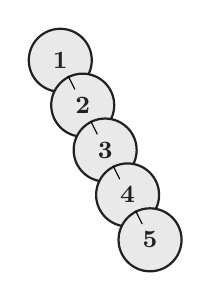
\begin{tikzpicture}[scale=0.38]
                \node[blacknode] {1}
                    child[missing] {}
                    child {node[blacknode] {2}
                        child[missing] {}
                        child {node[blacknode] {3}
                            child[missing] {}
                            child {node[blacknode] {4}
                                child[missing] {}
                                child {node[blacknode] {5}}
                            }
                        }
                    };
            \end{tikzpicture}
        \end{center}
        \begin{alertblock}{\faIcon{times-circle}\; Bad}
            Height $= 5$ \textbullet{} Degenerate \textbullet{} $O(n)$ ops
        \end{alertblock}

        \column{0.5\textwidth}
        \begin{center}
            \textbf{Red-Black Tree}\\[0.2cm]
            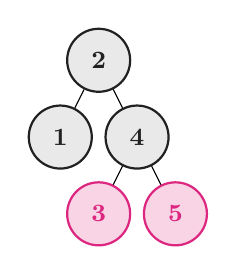
\begin{tikzpicture}[scale=0.65]
                \node[blacknode] {2}
                    child {node[blacknode] {1}}
                    child {node[blacknode] {4}
                        child {node[rednode] {3}}
                        child {node[rednode] {5}}
                    };
            \end{tikzpicture}
        \end{center}
        \begin{block}{\faIcon{check-circle}\; Excellent!}
            Height $= 3$ \textbullet{} Balanced \textbullet{} $O(\log n)$ ops
        \end{block}
    \end{columns}

    \pause
    \vspace{0.3cm}
    \begin{center}
        \Huge\textcolor{green!60!black}{\faIcon{check-circle}}\;
        \textbf{Self-Balancing Magic!}\;
        \textcolor{green!60!black}{\faIcon{magic}}
    \end{center}
\end{frame}


% Part 2b: Deletion
% ============================================================
% part2b_deletion.tex  –  Red-Black Tree: Deletion
% ============================================================

% ── Deletion intro ─────────────────────────────────────────
\begin{frame}{Deletion: Even More Fun!}
    \begin{center}
        \Large\textbf{Deletion is even more\ldots\ interesting!} \faIcon{smile}
    \end{center}

    \pause

    \begin{columns}
        \column{0.5\textwidth}
        \begin{center}
            \textbf{Deleting a \textcolor{rbred}{RED} node}
        \end{center}
        \begin{itemize}
            \item No problem!
            \item Just remove it
            \item Properties still hold
        \end{itemize}

        \column{0.5\textwidth}
        \pause
        \begin{center}
            \textbf{Deleting a \textbf{BLACK} node}
        \end{center}
        \begin{itemize}
            \item Oh boy\ldots
            \item Black height changes!
            \item Need ``double black'' fix
            \item Complex cases
        \end{itemize}
    \end{columns}

    \pause
    \vspace{0.4cm}
    \begin{center}
        \Large\textbf{Let's see both cases\ldots}
    \end{center}
\end{frame}

% ── Deletion Decision Flowchart (HORIZONTAL LAYOUT) ──────────
\begin{frame}{Deletion Decision Flowchart}
    \vspace{0.1cm}
    \begin{center}
    \begin{tikzpicture}[scale=0.8, every node/.style={transform shape},
        node distance = 0.6cm and 1.2cm,
        decision/.style = {diamond, draw=blue!60, fill=blue!12,
                           text width=3.5em, text centered,
                           inner sep=0pt, minimum height=2.3em,
                           font=\scriptsize},
        action/.style   = {rectangle, draw=green!60!black, fill=green!12,
                           text width=4.5em, text centered,
                           rounded corners=3pt, minimum height=1.8em,
                           font=\scriptsize},
        problem/.style  = {rectangle, draw=red!60, fill=red!12,
                           text width=4.5em, text centered,
                           rounded corners=3pt, minimum height=1.8em,
                           font=\scriptsize},
        arrow/.style    = {thick,->,>=stealth}]

        % Start node
        \node[decision] (del) {Delete\\Node};
        \node[decision, right=1.5cm of del] (isred) {Is node\\RED?};

        % TOP branch (YES - RED node - easy path)
        \node[action, above right=0.3cm and 1.2cm of isred] (remove) {Simply\\Remove};
        \node[action, right=0.8cm of remove] (done1) {\faIcon{check}\\Done!};

        % BOTTOM branch (NO - BLACK node - hard path)
        \node[problem, below right=0.3cm and 1.2cm of isred] (black) {BLACK\\Node};
        \node[decision, right=0.8cm of black] (sibling) {Check\\Sibling};
        \node[problem, right=0.8cm of sibling] (cases) {Apply\\4 Cases};
        \node[action, right=0.8cm of cases] (done2) {Rebalance\\\faIcon{check}};

        % Arrows
        \draw[arrow] (del) -- (isred);
        \draw[arrow] (isred) |- node[above,near start,font=\tiny]{Yes} (remove);
        \draw[arrow] (remove) -- (done1);
        \draw[arrow] (isred) |- node[below,near start,font=\tiny]{No} (black);
        \draw[arrow] (black) -- (sibling);
        \draw[arrow] (sibling) -- (cases);
        \draw[arrow] (cases) -- (done2);
    \end{tikzpicture}
    \end{center}

    \vspace{0.3cm}
    \begin{center}
        \textcolor{green!60!black}{\textbf{Top path (RED)}} = easy \quad
        \textcolor{red!60}{\textbf{Bottom path (BLACK)}} = complex
    \end{center}
\end{frame}

% ── Easy case: Deleting RED node ───────────────────────────
\begin{frame}{Case 1: Deleting a \textcolor{rbred}{RED} Node (Easy!)}
    \begin{center}
        \Large Delete \textbf{5} from our tree
    \end{center}

    \vspace{0.3cm}

    \begin{columns}
        \column{0.5\textwidth}
        \begin{center}
            \textbf{Before}\\[0.25cm]
            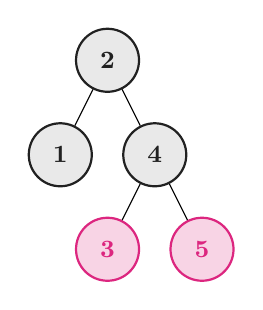
\begin{tikzpicture}[scale=0.8]
                \node[blacknode] {2}
                    child {node[blacknode] {1}}
                    child {node[blacknode] {4}
                        child {node[rednode] {3}}
                        child {node[rednode] {5}}
                    };
            \end{tikzpicture}
        \end{center}

        \column{0.5\textwidth}
        \pause
        \begin{center}
            \textbf{After}\\[0.25cm]
            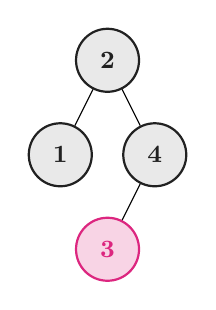
\begin{tikzpicture}[scale=0.8]
                \node[blacknode] {2}
                    child {node[blacknode] {1}}
                    child {node[blacknode] {4}
                        child {node[rednode] {3}}
                        child[missing] {}
                    };
            \end{tikzpicture}
        \end{center}
    \end{columns}

    \vspace{0.3cm}
    \pause

    \begin{center}
        \textbf{Why It's Easy}
    \end{center}
    \begin{itemize}
        \item Node 5 is \textcolor{rbred}{RED} and a leaf
        \item Simply remove it — black-height unchanged on all paths
        \item All properties still satisfied!
    \end{itemize}

    \pause
    \begin{center}
        \Large\textcolor{green!60!black}{\faIcon{check}}\; Done! That was nice!
    \end{center}
\end{frame}

% ── Hard case: Deleting BLACK node ─────────────────────────
\begin{frame}{Case 2: Deleting a \textbf{BLACK} Node (Uh oh\ldots)}
    \begin{center}
        \Large Delete \textbf{1} from our tree
    \end{center}

    \vspace{0.2cm}

    \begin{columns}
        \column{0.33\textwidth}
        \begin{center}
            \textbf{Before}\\[0.15cm]
            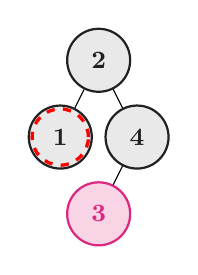
\begin{tikzpicture}[scale=0.65]
                \node[blacknode] (n2) {2}
                    child {node[blacknode] (n1) {1}}
                    child {node[blacknode] (n4) {4}
                        child {node[rednode] {3}}
                        child[missing] {}
                    };
                \draw[red, very thick, dashed] (n1) circle (0.55cm);
            \end{tikzpicture}
        \end{center}

        \column{0.33\textwidth}
        \pause
        \begin{center}
            \textbf{After Delete}\\[0.15cm]
            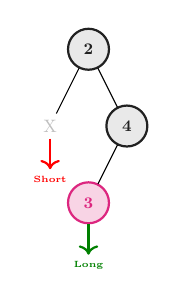
\begin{tikzpicture}[scale=0.65, every node/.style={transform shape}]
                \node[blacknode] (root) {2}
                    child {node[draw=none,fill=none,text=gray!50] (left) {X}} % X is the double-black placeholder
                    child {node[blacknode] (right) {4}
                        child {node[rednode] (r3) {3}}
                        child[missing] {}
                    };
                
                % Stable Arrow for Short Path (Left)
                \draw[->,thick,red] (left.south) -- ++(0,-0.6) 
                    node[below, font=\tiny\bfseries] {Short};
                    
                % Stable Arrow for Long Path (Right)
                \draw[->,thick,green!50!black] (r3.south) -- ++(0,-0.6) 
                    node[below, font=\tiny\bfseries]{Long};
            \end{tikzpicture}\\[0.1cm]
            \fcolorbox{red!80!black}{red!15}{\textcolor{red!70!black}{\bfseries\footnotesize\faIcon{times}~IMBALANCED}}
        \end{center}

        \column{0.33\textwidth}
        \pause
        \begin{center}
            \textbf{After Fix}\\[0.15cm]
            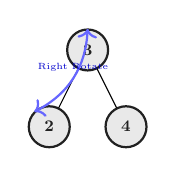
\begin{tikzpicture}[scale=0.65, every node/.style={transform shape}]
                % The balanced result after rotation and recoloring
                \node[blacknode] (n3) {3}
                    child {node[blacknode] (n2) {2}}
                    child {node[blacknode] (n4) {4}};

                % Annotation for the rotation
                \draw[<->, bend left, thick, blue!60] (n3.north) to node[above, font=\tiny, text=blue!80!black] {Right Rotate} (n2.north west);
                
            \end{tikzpicture}\\[0.1cm]
            
            % Status Box
            \fcolorbox{green!60!black}{green!15}{%
                \textcolor{green!50!black}{\bfseries\footnotesize\faIcon{check-circle}~BALANCED}%
            }
            
            % Specific actions taken
            \vspace{0.2cm}
            \begin{itemize}
                \item {\tiny \faIcon{sync} \textbf{Rotate:} Right at 4, then 2}
                \item {\tiny \faIcon{paint-brush} \textbf{Recolor:} 3 $\to$ Black}
            \end{itemize}
        \end{center}
    \end{columns}

    \vspace{0.2cm}
    \pause
\end{frame}


\begin{frame}{Black Node Deletion: The 4 Cases}
    % Compact tree styling - shorter and wider
    \tikzset{
        every node/.style={transform shape, scale=0.35},
        level distance=12mm,
        sibling distance=8mm,
        highlight/.style={draw=blue, ultra thick, inner sep=1pt},
        ghost/.style={opacity=0.3}
    }

    \vspace{-0.2cm}

    % Using top-aligned columns for better vertical distribution
    \begin{columns}[t, onlytextwidth]
        % --- LEFT COLUMN ---
        \column{0.48\textwidth}
        \begin{block}{Case 1: Sibling RED}<1->
            \vspace{-0.25cm}
            \centering
            \begin{tikzpicture}[level distance=10mm, sibling distance=7mm]
                \node[blacknode] {P}
                    child {node[blacknode, ghost] {X}}
                    child {node[rednode, highlight] {S} 
                        child {node[blacknode] {L}}
                        child {node[blacknode] {R}}
                    };
            \end{tikzpicture}\\[-0.1cm]
            {\tiny Rotate \& Recolor \faIcon{sync}}
            \vspace{-0.25cm}
        \end{block}

        \vspace{0.1cm}

        \begin{block}{Case 3: Left RED}<3->
            \vspace{-0.25cm}
            \centering
            \begin{tikzpicture}[level distance=10mm, sibling distance=7mm]
                \node[blacknode] {P}
                    child {node[blacknode, ghost] {X}}
                    child {node[blacknode] {S}
                        child {node[rednode, highlight] {L}}
                        child {node[blacknode] {R}}
                    };
            \end{tikzpicture}\\[-0.1cm]
            {\tiny Right-rotate at S \faIcon{redo}}
            \vspace{-0.25cm}
        \end{block}

        % --- RIGHT COLUMN ---
        \column{0.48\textwidth}
        \begin{block}{Case 2: All BLACK}<2->
            \vspace{-0.25cm}
            \centering
            \begin{tikzpicture}[level distance=10mm, sibling distance=7mm]
                \node[blacknode] {P}
                    child {node[blacknode, ghost] {X}}
                    child {node[blacknode, highlight] {S}
                        child {node[blacknode] {L}}
                        child {node[blacknode] {R}}
                    };
            \end{tikzpicture}\\[-0.1cm]
            {\tiny Recolor S to RED \faIcon{paint-brush}}
            \vspace{-0.25cm}
        \end{block}

        \vspace{0.1cm}

        \begin{block}{Case 4: Right RED}<4->
            \vspace{-0.25cm}
            \centering
            \begin{tikzpicture}[level distance=10mm, sibling distance=7mm]
                \node[blacknode] {P}
                    child {node[blacknode, ghost] {X}}
                    child {node[blacknode] {S}
                        child {node[blacknode] {L}}
                        child {node[rednode, highlight] {R}}
                    };
            \end{tikzpicture}\\[-0.1cm]
            {\tiny Left-rotate at P \faIcon{undo}}
            \vspace{-0.25cm}
        \end{block}
    \end{columns}

    % Goal footer only appears on final step to save space initially
    \only<5->{
        \vspace{0.1cm}
        \begin{center}
            {\tiny\faIcon{lightbulb} Goal: Move RED to short path or recolor}
        \end{center}
    }
\end{frame}


% Part 3: Applications and Conclusion
% Real-world applications
\begin{frame}{Where Are Red-Black Trees Used?}
    \begin{center}
        \Large\textbf{Everywhere!}
    \end{center}
    
    \pause
    
    \begin{columns}
        \column{0.5\textwidth}
        \begin{itemize}
            \item<2-> \faIcon{linux} \textbf{Linux Kernel}\\
                \small Process scheduling
            \item<3-> \faIcon{java} \textbf{Java}\\
                \small TreeMap, TreeSet
            \item<4-> \faIcon{database} \textbf{Databases}\\
                \small Indexing structures
            \item<5-> \faIcon{folder} \textbf{File Systems}\\
                \small Directory organization
        \end{itemize}
        
        \column{0.5\textwidth}
        \only<6->{
            \begin{center}
                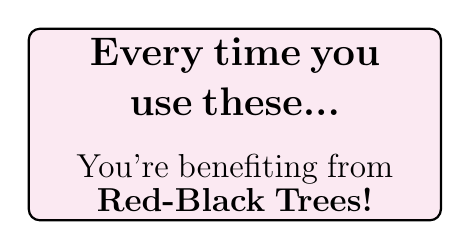
\begin{tikzpicture}
                    \node[draw, thick, rounded corners, fill=rbred!10, text width=5cm, align=center, minimum height=2cm] {
                        \Large\textbf{Every time you use these...}\\[0.3cm]
                        \large You're benefiting from\\
                        \textbf{Red-Black Trees!}
                    };
                \end{tikzpicture}
            \end{center}
        }
    \end{columns}
\end{frame}

% Conclusion
\begin{frame}{So There You Have It!}
    \begin{center}
        \Large\textbf{Red-Black Trees in a Nutshell}
    \end{center}
    
    \pause
    
    \begin{columns}
        \column{0.6\textwidth}
        \begin{itemize}
            \item<2-> Complex but incredibly powerful
            \item<3-> Tricky to implement
            \item<4-> Guaranteed $O(\log n)$ performance
            \item<5-> Used everywhere in computing
        \end{itemize}
        
        \column{0.4\textwidth}
        \only<6->{
            \begin{center}
                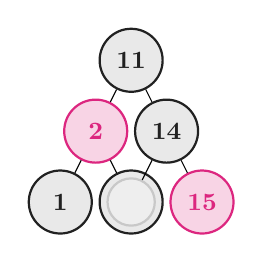
\begin{tikzpicture}[scale=0.6]
                    \node[blacknode] {11}
                        child {node[rednode] {2}
                            child {node[blacknode] {1}}
                            child {node[blacknode] {7}}
                        }
                        child {node[blacknode] {14}
                            child {node[nilnode] {}}
                            child {node[rednode] {15}}
                        };
                \end{tikzpicture}
            \end{center}
        }
    \end{columns}
    
    \pause[7]
    
    \vspace{0.5cm}
    
    \begin{center}
        \begin{alertblock}{Remember}
            The next time you're struggling with RBT implementation...\\[0.3cm]
            \large Even the \textbf{inventor} moved on to Left-Leaning Red-Black Trees! \faIcon{laugh}
        \end{alertblock}
    \end{center}
    
    \pause
    
    \begin{center}
        \Large\textbf{Thanks for listening!}\\[0.3cm]
        \large May your trees always stay balanced! \faIcon{tree}
    \end{center}
\end{frame}

% Questions slide
\begin{frame}
    \begin{center}
        \Huge\textbf{Any Questions?}\\[1cm]
        \Large\faIcon{comments}
    \end{center}
\end{frame}


\end{document}
